%!TEX root = ../thesis.tex
%*******************************************************************************
%*********************************** First Chapter *****************************
%*******************************************************************************

\chapter{Introduction}  %Title of the First Chapter

\ifpdf
    \graphicspath{{Chapter1/Figs/Raster/}{Chapter1/Figs/PDF/}{Chapter1/Figs/}}
\else
    \graphicspath{{Chapter1/Figs/Vector/}{Chapter1/Figs/}}
\fi

\section{Breaking the diffraction limit reveals structure below 200\,nm}
Our understanding of the biology of life is limited to what we can observe. 
Naked human vision is limited to a spatial resolution on the order of \SI{100}{\micro\metre}~\cite{devalois1990spatial}.
The invention of high power microscopes, often attributed to van Leeuwenhoek in 1660~\cite{van1800select}, and pioneering experiments by Robert Hooke~\cite{hooke1667micrographia} and Swammerdam~\cite{swammerdam1758book} around the same time, revealed phenomena previously invisible to the naked human eye. 

Lens technology continuously improved through the 17\textsuperscript{th} and 18\textsuperscript{th} Centuries~\cite{dollond1753xiv, daumas1972scientific}, revealing smaller and smaller objects, until in 1873 Abbe showed that the diffraction of light as it passes through a lens places a fundamental limit on the size of objects which can be resolved~\cite{abbe1873beitrage}. The famous Abbe diffraction limit, given in Equation~\ref{eq:abbe}, states that the minimum separation distance, $d$, at which two objects can be resolved decreases with the wavelength of light, $\lambda$, but increases with the lens' acceptance angle, $\alpha$, and refractive index of the medium between the lens and the object, $n$. The wavelength range of visible light is \SIrange[range-phrase=--]{400}{700}{\nano\metre}, and the maximum acceptance angle of a lens approaches \SI{90}{\degree}. The refractive index of air is $1.0$, although special immersion oils can be used to increase $n$ to \textasciitilde\num{1.5}. Using Equation~\ref{eq:abbe}, we then calculate that the maximum resolution of a microscope lens is \textasciitilde\SI{200}{\nano\metre}. 

\begin{equation} \label{eq:abbe}
d = \frac{\lambda}{2n\sin\left (\alpha  \right )}\end{equation}

A number of technologies which are not based on visible light exist to greatly surpass the resolution of optical microscopes, including transmission electron microscopy and scanning electron microscopy~\cite{reinhold1931configuration, wells2006early, reimer2013transmission}.
However these techniques require sample preparation which includes a combination of freezing, fixation, or toxic staining~\cite{kuo2007electron}; must image the sample under vacuum conditions at cryogenic temperatures; and use a minimum electron dose which is lethal to cells~\cite{de2016live}. 
Electron microscopy is therefore incompatible with live cell biology.

Furthermore, the invention of fluorescent labelling gives optical microscopy a distinct advantage over any other microscopy technique in terms of specificity. 
Sophisticated biochemistry, based on antibody chemistry, genetic expression, and other biotechnologies, can be used to label specific cellular compartments or organelles with fluorescent molecules~\cite{day2014fluorescent}. 
When these fluorescent molecules are illuminated with a certain wavelength of light, they absorb photons, exciting electrons to a higher electronic energy state~\cite[\textit{ch. 1}]{lakowicz2007principles}. 
The electrons lose some energy through so-called vibrational states, then as the electron falls back to the ground electronic state photons are emitted at a red-shifted wavelength - where the wavelength shift is proportional to the energy lost through the vibrational states, as per the Plank-Einstein relation $E=h\nu=hc/\lambda$~\cite[\textit{ch. 39}]{halliday2010principles}. 

Fluorescent labelling has a number of unique applications. 
Firstly, since the light used to excite fluorescence is blocked by filters before it reaches the observer, only fluorescence emission light is seen through the microscope~\cite{ploem1967use}. 
This creates a high-contrast image showing the object of interest against a black background. 
Furthermore the specificity of labelling means that other parts of the cell which are not of interest for a given experiment are invisible, further enhancing the observability of the labelled target~\cite{day2014fluorescent}.
Finally, if two or more fluorescent labels are used with non-overlapping fluorescent spectra, then imaging in multiple channels can be used for colocalisation studies, for example to confirm that a certain protein interacts with a certain organelle~\cite{dunn2011practical}. 

The unique advantages of fluorescent labelling have motivated researchers in the last two decades to invent optical methods to image at resolutions below the diffraction limit~\cite{cornea2014fluorescence}.
Whilst it remains impossible to capture an individual image beyond the diffraction limit, digital cameras and intensive computational reconstruction have enabled techniques which sacrifice temporal resolution for enhanced spatial resolution.
This is the principle behind techniques based on photoactivated localisation microscopy (PALM)~\cite{betzig2006imaging} and stochastic optical reconstruction microscopy (STORM)~\cite{rust2006sub}: in each image, only a small fraction - typically less than \SI{1}{\percent} - of fluorophores are emitting light.
Multiple images are captured so that the molecules blink in a video of the raw data; assuming that two adjacent fluorophores do not emit simultaneously, the centre of the diffraction pattern is calculated as the true location of the molecule. 
When enough frames have been captured for every fluorescent molecule to have a high probability of emitting - for example, 1000\,frames for a \SI{1}{\percent} duty cycle - the localisation algorithm is applied to every image in the dataset, and a super-resolution image can be constructed. 

In STORM microscopy, there is a trade-off between spatial resolution and acquisition time; a lower duty cycle with more frames captured will produce a higher spatial resolution, as there is a lower probability of two adjacent fluorescent molecules emitting simultaneously. 
In practice, STORM has been shown to achieve a spatial resolution of \textasciitilde\SIrange[range-phrase=--]{10}{20}{\nano\metre}; however resolutions in this range typically require \SIrange[range-phrase=--]{1}{5}{\minute} of imaging to capture the data for a single reconstructed super-resolution image~\cite{heilemann2008subdiffraction}.
Dynamic events in live cell biology cannot be captured, and so a faster technique must be used for such experiments. 

Structured illumination microscopy (SIM) can produce a resolution-enhanced image beyond the diffraction limt with just 9 raw images~\cite{gustafsson2000surpassing}.
The technique is described in detail in Chapter~\ref{chap:LAGSIM}, which explains how computational reconstruction produces an image with twice the resolution of a widefield image captured with the same lens. 
Using state-of-the-art lenses and cameras, we have shown SIM datasets with a spatial resolution of <\SI{90}{\nano\metre}, at a video rate of \SI{11}{\hertz}~\cite{young2016guide}.   

\section{Microscopy in 3D provides a deeper biological understanding}
Capturing 2-dimensional (2D) images of microscopic biology has enhanced our understanding of life and disease, enabling development of new medicines and diagnosis techniques. 
However human biology is made up of inherently 3-dimensional (3D) structures, from the sub-cellular scale to the full body. 

Other fields of medicine have shown the advantages offered by capturing 3D information; for example, compare a 2D x-ray image with a 3D computed tomography (CT) dataset. 
Whilst the former can be used for detecting breaks in bones or confirming the presence of foreign objects in the body~\cite{markose2009three}, the extra information provided by 3D data significantly improves diagnosis and treatment planning in ocology and trauma by accurately modelling tumours~\cite{zhang2013thin} or fractures~\cite{rangarajan2013three}. 

In widefield epifluorescent microscopy, out-of-focus light makes visualising 3D reconstructions futile, as light emitting from a given axial position obscures structures in other focal planes of the lens. 
To accurately represent fluorescent objects in 3 dimensions, an optical section must be captured - that is, a clear image deep in the sample without out-of-focus light.
Several optical sections can then be gathered at a number of depths to build up a 3-dimensional dataset. 

A number of modern microscopy techniques are able to perform optical sectioning. 
Confocal microscopy is a point-scanning technique which uses a pinhole in the emission path to remove out-of-focus light, building up an optically-sectioned image pixel-by-pixel~\cite{white1987evaluation, marvin1961microscopy}. 
Single plane illumination microscopy (SPIM) uses one objective to generate a thin sheet of light in the sample which is imaged by a second orthogonal objective, providing optical sectioning physically by not generating out-of-focus light in the first place~\cite{huisken2004optical}. 
Optical projection tomography (OPT) can be thought of as the optical analogue of x-ray computerised tomography, capturing images at several rotations of the sample and using the inverse Radon transform to reconstruct a 3-dimension dataset~\cite{sharpe2002optical}. 
Structured illumination microscopy (SIM) uses pattered illumination light to computationally remove out-of-focus light, which can also provide resolution enhancement, detailed in Chapter~\ref{chap:LAGSIM}. 
Several techniques exist for 3D localisation microscopy, utilising one or more of astigmatism~\cite{huang2008three}, double-helix point-spread function (PSF) engineering~\cite{pavani2009three}, dual-lens interferometry~\cite{shtengel2009interferometric}, multiple focus planes~\cite{toprak2007three}, and Airy beams~\cite{jia2014isotropic}; these techniques report typical resolutions of \SIrange[range-phrase=--]{10}{30}{\nano\metre} in 3 dimensions. 

An online tool for visualising and sharing such information-rich volumetric dataasets is presented in Chapter~\ref{chap:FPB}. 

\section{Cell biology for microscopy}
The tools described in Chapters~\ref{chap:LAGSIM} and \ref{chap:FPB} have valuable applications in cell biology, which are detailed in Chapters~\ref{chap:MOF} and \ref{chap:ER}.
Since this thesis covers a broad range of themes, from engineering through computer science to biology, this section is included to provide a background of cell biology necessary for appreciating the findings detailed in the application chapters. 

\subsection{Labelling organelles to visualise cell location}
Figure~\ref{fig:animal-cell} shows a generic animal cell~\cite{wikicell}. 
Highlighted in colour are 8 organelles which are investigated in work presented throughout this thesis. 
The scale and quoted sizes are approximate, included to convey which organelles are resolvable in standard widefield microscopy, and which are smaller than the diffraction limit requiring super-resolution to observe clearly. 

\begin{figure}[htbp!]
\centering
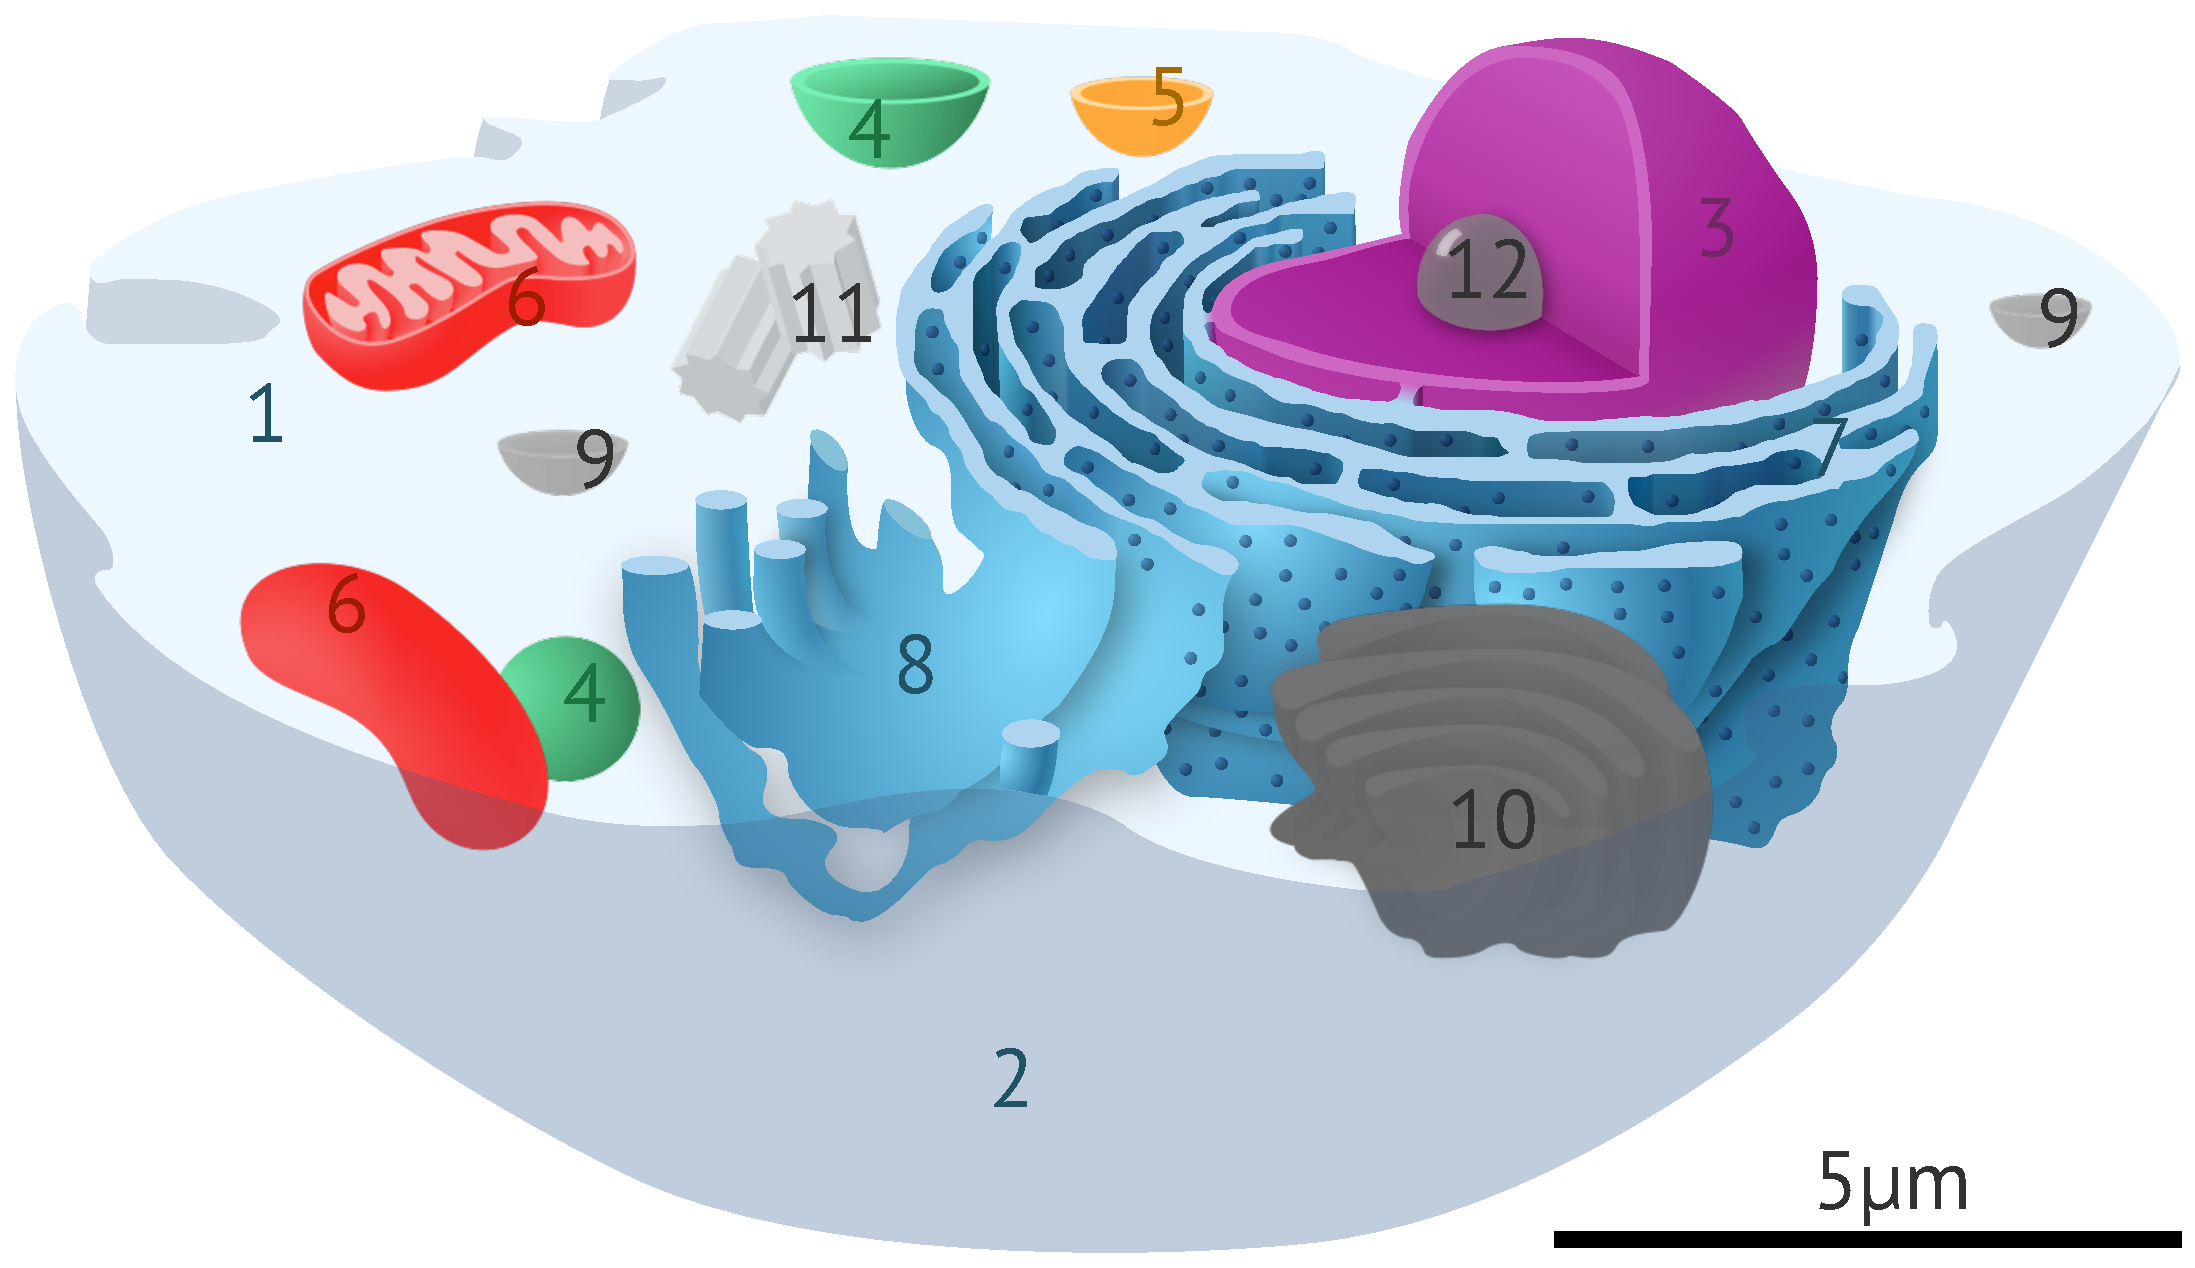
\includegraphics[width=1.0\textwidth]{animal-cell}
\captionsetup{singlelinecheck=off}
\caption[Introduction: Animal cell labelled with organelles relevant to this thesis]{A generic animal cell, adapted from Wikipedia~\cite{wikicell}, but with the organelles discussed in this thesis highlighted in colour. Scalebar is approximate: most animal cells are \SIrange[range-phrase=--]{10}{30}{\micro\metre} in diameter. Numbered annotations with approximate sizes from~\cite{hammersen2002histology} are as follows:\newline 

\begin{tabular}{p{1em}p{0.2\textwidth}p{0.5\textwidth}}
	1. & Cytosol  &\SIrange[range-phrase=--]{10}{30}{\micro\metre} diameter \\
	2. & Cell membrane  &\SI{1}{\nano\metre} thick \\
	3. & Nucleus  &\SI{6}{\micro\metre} diameter (average) \\
	4. & Lysosome  &\SIrange[range-phrase=--]{0.1}{1.2}{\micro\metre} \\
	5. & Endosome  &\SIrange[range-phrase=--]{0.05}{1}{\micro\metre} \\
	6. & Mitochondria  &\SI{250}{\nano\metre} wide, \SIrange[range-phrase=--]{2}{7}{\micro\metre} long \\
	7. & ER network  &\SIrange[range-phrase=--]{30}{100}{\nano\metre} diameter \\
	8. & ER sheets  &\SIrange[range-phrase=--]{40}{70}{\nano\metre} thick \\
	9. & Vesicle  &\SIrange[range-phrase=--]{200}{300}{\nano\metre} diameter \\
	10. & Golgi apparatus  &\SIrange[range-phrase=--]{1}{2}{\micro\metre} wide \\
	11. & Centrosome  &\SI{200}{\nano\metre} diameter \\
	12. & Nucleolus  &\SIrange[range-phrase=--]{2}{4}{\micro\metre} diameter 
\end{tabular} } % end of caption!
\label{fig:animal-cell}
\end{figure} 

Each of the organelles highlighted in Figure~\ref{fig:animal-cell} can be labelled with a fluorescent marker.
Fluorescent labelling can provide a variety of information about the cell, depending on the function of the organelles of interest~\cite{day2014fluorescent}. 

The cell nucleus contains DNA, the genetic code of life~\cite{alberts2002molecular}, and can be visualised under a microscope by labelling with dyes such as DAPI or SiR-DNA~\cite{kapuscinski1995dapi, lukinavivcius2015sir}. 
Labelling the nucleus provides an easy method of automated cell counting, or an easy method for locating cells if it is not clear from other labels~\cite{porter1980use}. 

The contents of the cell are contained by the cell membrane, which acts as a barrier between the contents of the cell and extra-cellular space~\cite[\textit{ch. 1}]{alberts2013essential}. 
Membrane proteins can be specifically labelled to visualise the outline of cells, to confirm whether another fluorescent object is located inside or outside of the cell~\cite{yano2009tag, lee2011fluorescent, chamma2017optimized}. 

\subsection{Labelling membrane structures to observe endocytosis}
The cell can import useful raw materials through the membrane by a process called endocytosis~\cite{alberts2002molecular}. 
To enter the cell, an intracellular compartment is created from the plasma membrane to contain the foreign material.
Once inside the cell, there are many pathways for processing the endocytosed contents~\cite{marsh2001endocytosis, marsh1999structural, mcmahon2011molecular}. 
A typical pathway, shown in Figure~\ref{fig:endocytosis-pathway}, imports contents into small vesicles called early endosomes, which are selectively sorted to either recycle the contents to the cell membrane or develop into late endosomes. 
Late endosomes have an acidic environment, about pH\,\num{5.5}, and begin hydrolytic digestion of their contents~\cite{geisow1984ph}. 
Late endosomes mature into lysosomes with a more acidic environment and enzymes which further break down their contents~\cite{alberts2002molecular}. 
Labelling endosomes or lysosomes alongside other objects can be used for colocalisation studies, as performed in Chapter~\ref{chap:MOF}, which show whether another fluorescent substance is contained within the organelle or is moving freely in the cytosol~\cite{pike2017quantifying}. 

\begin{figure}[!b]
\centering
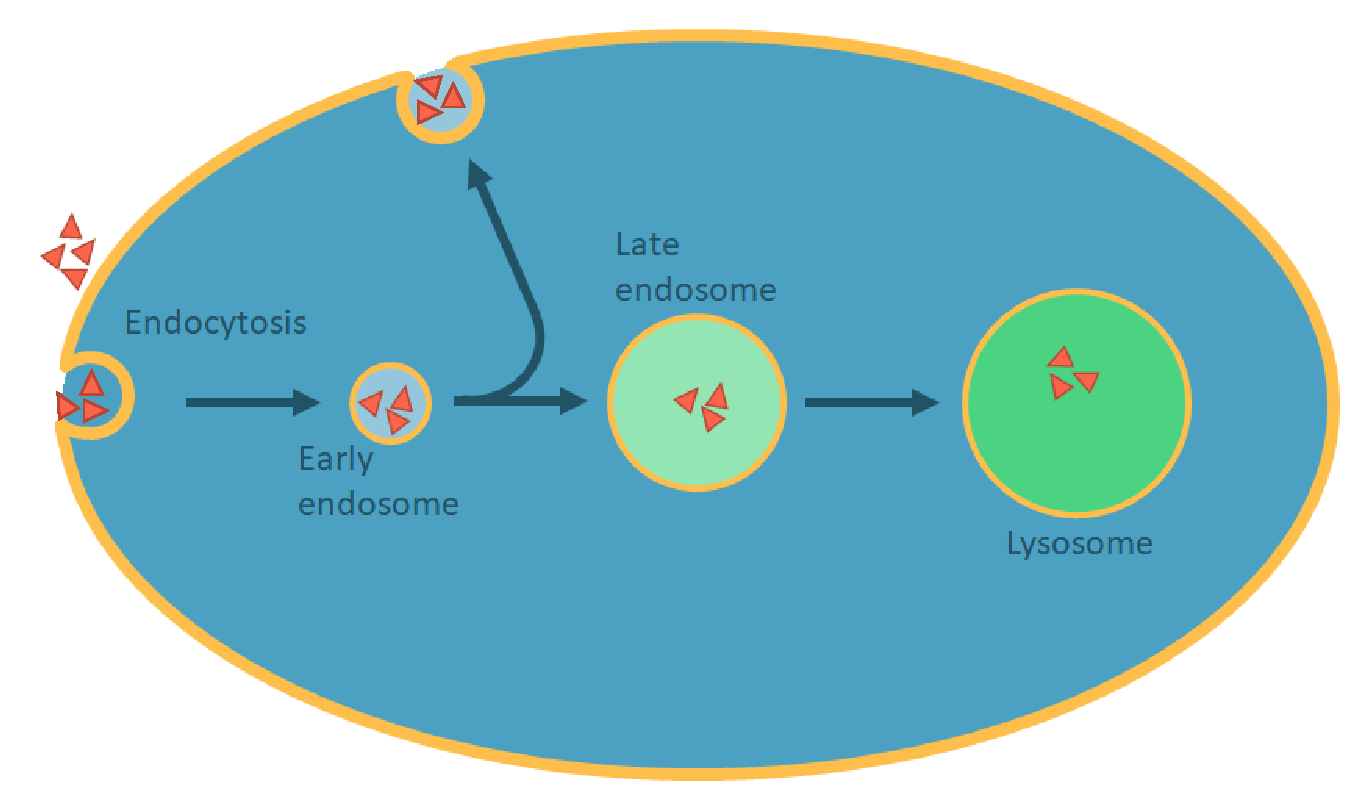
\includegraphics[width=1.0\textwidth]{endocytosis-pathway}
\captionsetup{singlelinecheck=off}
\caption[Introduction: Cells import external contents through endocytosis]{A typical endocytosis pathway shows the formation of various organelles, each of which contains a different environment for ingestion and processing of the external contents. Other endocytosis pathways also occur, for example to pass the contents to ER or release it directly into the cytosol. Figure adapted from ~\cite{alberts2002molecular}. } 
\label{fig:endocytosis-pathway}
\end{figure}

In addition to endosomes and lysosomes, other internal membrane structures include the endoplasmic reticulum (ER) and the Golgi apparatus. 
Protein folding and synthesis occurs in the ER; conversely, the Golgi apparatus is involved in further protein processing and secretion of substances from the cell~\cite{dyson1978cell}. 
Content is transferred between all intracellular compartments, either through vesicles or by direct organelle-organelle interaction. 
To visualise the ER, fluorescent labels can be applied to either the ER membrane or to luminal proteins contained within the ER network~\cite{costantini2013probing}; both labelling techniques are utilised in Chapter~\ref{chap:ER}.  

\subsection{Labelling mitochondria to investigate energy-dependent processes and cancer}
Mitochondria generate energy for the cell by converting food to adenosine triphosphate (ATP), an energy-rich molecule that is used as the basic chemical fuel to power cellular activity~\cite{alberts2013essential}. 
This process, known as the Krebs cycle, consumes oxygen and produces carbon dioxide and water as waste products, so is a type of cellular respiration. 
Furthermore, mitochondria are responsible for triggering apoptosis - that is, controlled cell death~\cite{murray1993cell}. 

In cancerous cells the Krebs cycle is bypassed, and ATP is produced by a more direct process known as glycolysis~\cite{warburg1930uber}. 
By avoiding the Krebs cycle, cancer cells stop the mitochondria from triggering apoptosis, such that the cells become immortal and continuously
 reproduce to form tumours~\cite{murray1993cell}. 
Chapter~\ref{chap:MOF} uses fluorescently labelled  mitochondria to assess their interaction with a drug designed to restart the Krebs cycle in cancerous cells. 

All the organelles discussed so far are located in the cytosol, a crowded solution of many different types of molecules filling the volume of the cell~\cite{goodsell1991inside}. 
This solution is so dense that the cytosol behaves as a water-based gel rather than a liquid~\cite{alberts2013essential}. 

\subsection{Labelling the cytoskeleton shows cellular structure} \label{sec:cytoskeleton}
The cellular cytoskeleton is composed of long, fine protein filaments forming a system of girders, ropes, and motors to give the cell mechanical strength, control its shape, and drive movement~\cite{alberts2013essential}.
There are three types of filament: microtubules, actin, and intermediate filaments, as seen in Figure~\ref{fig:cytoskeleton}. 
Labelling these components with fluorescent markers provides a clear visualisation of the cell boundary, and shows strong colocalisation between filaments and other organelles~\cite{melkov2017regulation}. 
They are also often used as test samples to assess the performance of a microscope, for example determining resolution by measuring the minimum resolvable separation distance between two fibres~\cite{dyba2003immunofluorescence, wegel2016imaging}. 

\begin{figure}[htbp!]
\centering
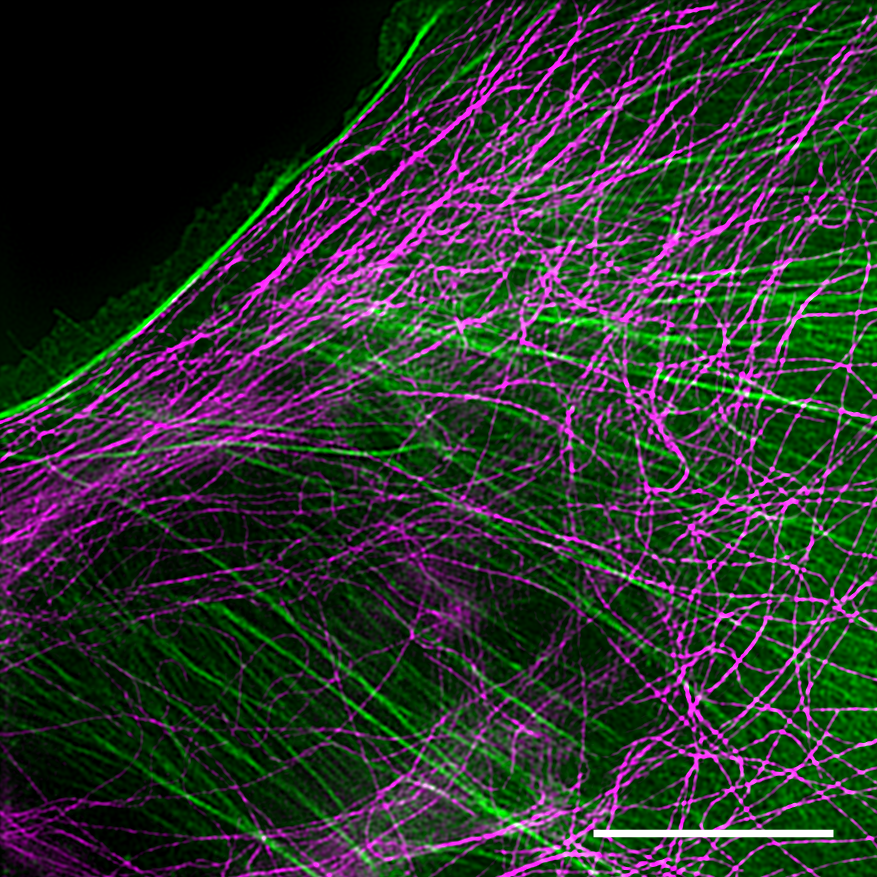
\includegraphics[width=1.0\textwidth]{cytoskeleton}
\caption[Introduction: The cytoskeleton gives the cell structure and strength]{The cytoskeleton is composed of actin filaments, shown in green, microtubules, shown in magenta, and intermediate filaments, not shown, which give the cell structure and strength. The sample shown is of commercial GATTA Cells 4C, imaged on LAG SIM. Scalebar is \SI{10}{\micro\metre}.}
\label{fig:cytoskeleton}
\end{figure}

\section{Aims and structure of this thesis}
Since October 2015, I have been working in the Laser Analytics Group building tools and applying them to answer biological questions. 

Chapter~\ref{chap:LAGSIM} describes the development a structured illumination microscope. 
SIM is a microscopy technique which generates images in the niche between STORM, which provides \SI{20}{\nano\metre} resolution but takes \SI{5}{\minute} or more per acquisition; and widefield microscopy, which can image at 100\,frames per second but at a diffraction limited resolution of about \SI{200}{\nano\metre}. 
The Laser Analytics Group's SIM (LAG SIM) achieves \SI{80}{\nano\metre} resolution at 11\,frames per second. 

As a relatively new invention, super-resolution microscopes are often difficult to use and require expert skill to achieve their optimal performance. 
An important aim for LAG SIM was that any researcher should be able to use it, with minimal training required for capturing and reconstructing SIM data. 
In Chapter 2, a showcase of reconstructed SIM data from a wide variety of experiments is provided as a reference for capturing high-quality images. 

Resolving microscopic biology in 3D reveals structures and events that would otherwise be invisible; for example, observing the development of a zebrafish embryo from 64 cells to \num{20000} cells~\cite{keller2008reconstruction}, or the 3D interaction of mitochondria with microtubules~\cite{huang2016ultra}. 
LAG SIM is able to capture 3D data using a capability known as optical sectioning.
Whilst this data is information-rich and exciting to explore in detail, sharing and publishing the datasets in an informative way presents a challenge to authors, who are restricted to showing 2D slices or projections of the data or videos from one perspective.
If readers were able to interact directly with the 3D volume they would gain a deeper understanding of the volumetric arrangement of structures.

To address this issue, Chapter~\ref{chap:FPB} presents FPBioimage, an online tool for sharing and publishing 3D volumetric data. 
A key aim again was that the software was easy to operate, so that non-expert users could effortlessly view or share data from and to anywhere in the world. 
In combination with a suite of additional software built to complement the main tool, FPBioimage makes sharing and publishing 3D volumetric data a one-click process.
The chapter describes the development of the software, and presents a wide assortment of data from different 3D imaging technologies highlighting the unique features of the tool. 

Chapter~\ref{chap:MOF} demonstrates the capability of LAG SIM for facilitating hypothesis-driven research, introducing the use of metal organic frameworks (MOFs) as drug delivery vehicles for treating cancer. 
Many potentially therapeutic drugs degrade quickly in extra-cellular media, either making them unsuitable for use as medicines or requiring a high dosage with unwelcome side-effects. 
Model drugs, including small-interfering ribonucleic acid (siRNA) and dichloroacetic acid (DCA), were loaded into the large pores of the MOF's crystalline structure, with the aim of protecting the contents for delivery into cells. 

The LAG SIM was used to image the uptake of the treatment over a time period of 24-hours, and 3-dimensional images have been published online with FPBioimage to allow other researchers to explore the data themselves and verify the results. 
Three biological experiments are described showing the therapeutic effects offered by this newly-developed technology. 

Chapter~\ref{chap:ER} utilises the fast, high-resolution imaging provided by LAG SIM to present pioneering discoveries about the endoplasmic reticulum (ER). 
It has recently been discovered that proteins within the ER move with directed flow, rather than diffusive motion which was previously assumed. 
Working in collaboration with the researchers who first discovered this phenomenon, LAG SIM's unique spatio-temporal resolution was utilised with the aim of finding the origin of directed luminal flow. 

High-speed videos reveal the ER membrane pinching at a high frequency, which was hypothesised to cause a peristaltic flow. 
Computational analysis is presented to understand and interpret experimental results, and compelling evidence is shown which advances the understanding of fundamental cell biology. 

Each chapter begins with its own detailed introduction to the topic, including background information and a review of relevant literature. 

Finally, a concluding Chapter~\ref{chap:conclusion} highlights the key discoveries and contributions made as part of this work.